% !TEX TS-program = xelatex
% !TEX encoding = UTF-8 Unicode
% !Mode:: "TeX:UTF-8"

\documentclass{resume}
\usepackage{zh_CN-Adobefonts_external} % Simplified Chinese Support using external fonts (./fonts/zh_CN-Adobe/)
% \usepackage{NotoSansSC_external}
% \usepackage{NotoSerifCJKsc_external}
% \usepackage{zh_CN-Adobefonts_internal} % Simplified Chinese Support using system fonts
\usepackage{linespacing_fix} % disable extra space before next section
\usepackage{cite}
\usepackage{tabu}
\usepackage{progressbar}
\usepackage{multirow}

\begin{document}
\pagenumbering{gobble} % suppress displaying page number
\Large{
  \begin{tabu}{ c l r }
    \multirow{4}{1in}{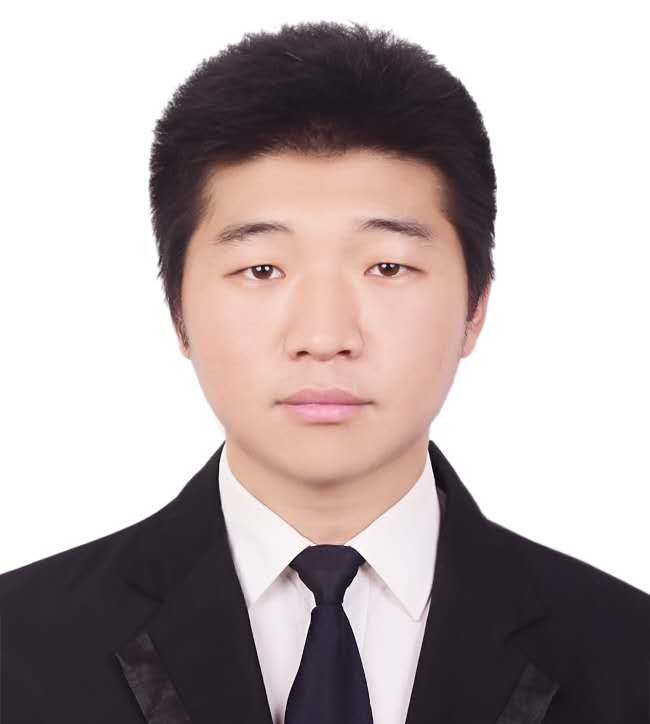
\includegraphics[width=1in]{profile}} & \scshape{高亚虎} & {Linux~}\progressbar{0.55} \\
    & \email{gao\_yahu@163.com} & {Python~}\progressbar{0.50} \\
    & \phone{(+86) 131-2029-0626\ \ \ \ } & {C~}\progressbar{0.5} \\
    & \github[github.com/yahugao]{https://github.com/yahugao} & {shell~}\progressbar{0.3}
  \end{tabu}
}

\section{\faUsers\ 工作经历}\normalsize
\datedsubsection{\textbf{瞬联软件科技有限公司}, 北京}{2017/09/20 -- 现在}
\role{系统工程师}{职责: windriver linux发行版的维护和升级}
\begin{itemize}
    \item {客户系统的维护,对客户在使用wind river Linux系统中的问题进行调查和修复}    
	\item {CVE漏洞的修复,根据客户的要求对NVD网站公布的软件漏洞在不同版本上进行修复}
    \item {工作中解决的主要的非CVE问题有(windriver linux平台):}
    \begin{itemize}
        \item {NFS文件系统的不能更新客户端创建文件的权限}
        \item {内核启动过程panic, 不能自动挂载NFS rootfs}
        \item {proc文件系统中潜在的Kernel NULL}
        \item {NFSv4 server端重启后,延迟响应客户端请求的原因}
        \item {ulimit 设置内存上限不生效}
    \end{itemize}
\end{itemize}

\section{\faUsers\ 实习经历}\normalsize
\datedsubsection{\textbf{英特尔(中国)有限公司} 北京}{2016年8月 -- 2017年2月}
\role{实习软件工程师}{职责: LTP(Linux test project)由PC端向移动端的移植与验证}
\begin{itemize}
    \item {主要收获:}
    \begin{itemize}
        \item {完成了LTP由PC向车载Android平台Brillo的移植,解决了LTP在平台迁移过程中的不兼容问题}
        \item {向LTP开源社区成功提交了修复数据类型的patch}
    \end{itemize}
\end{itemize}

\section{\faGraduationCap\  教育背景}\normalsize
\datedsubsection{\textbf{中国人民解放军信息工程大学}, 河南,郑州}{2014年9月 -- 2017年7月}
\role{硕士研究生}{专业:计算机科学与技术 方向:软件分析与逆向工程}
\begin{itemize}
    \item {主要成就:}
    \begin{itemize}
        \item {设计并实现了在动态二进制翻译过程中,对本地库函数的调用,极大的提升了动态二进制翻译系统的效率}
        \item {实现了C程序利用静态翻译生成的指令在目标平台的封装}
    \end{itemize}
\end{itemize}
\datedsubsection{\textbf{河北理工大学}, 河北, 唐山}{2010年9月 -- 2014年7月}
\role{学士}{专业:计算机科学与技术}
%\datedsubsection{\textbf{\LaTeX\ 简历模板}}{2015 年5月 -- 至今}
%\role{\LaTeX, Python}{个人项目}
%\begin{onehalfspacing}
%优雅的 \LaTeX\ 简历模板, https://github.com/billryan/resume
%\begin{itemize}
%  \item 容易定制和扩展
%  \item 完善的 Unicode 字体支持,使用 \XeLaTeX\ 编译
%  \item 支持 FontAwesome 4.5.0
%\end{itemize}
%\end{onehalfspacing}

% Reference Test
%\datedsubsection{\textbf{Paper Title\cite{zaharia2012resilient}}}{May. 2015}
%An xxx optimized for xxx\cite{verma2015large}
%\begin{itemize}
%  \item main contribution
%\end{itemize}


\section{\faCogs\ IT 技能}\normalsize
% increase linespacing [parsep=0.5ex]
\begin{itemize}[parsep=0.5ex]
  \item {编程语言: C == Python > Java > C++}
  \item 平台: Linux
  \item 工具: Yocto,rpm,vim
\end{itemize}
%\datedsubsection{\textbf{COURSERA 认证}}{2018年10月}
%\begin{itemize}[parsep=0.5ex]
%	\item 证书名称: Machine Learning
%	\item 证书编号: NFCZEBTZ5T4L
%	\item 证书URL : https://www.coursera.org/account/accomplishments/verify/NFCZEBTZ5T4L
%\end{itemize}


%\section{\faHeartO\ 获奖情况}
%\datedline{\textit{第一名}, xxx 比赛}{2013 年6 月}
%\datedline{其他奖项}{2015}

\section{\faInfo\ 其他}\normalsize
% increase linespacing [parsep=0.5ex]
\begin{itemize}[parsep=0.5ex]
  \item GitHub: https://github.com/gyher
  \item 语言: 英语 - 熟练(CET-4)
  \item 爱好:跑步,健身
\end{itemize}

%% Reference
%\newpage
%\bibliographystyle{IEEETran}
%\bibliography{mycite}
\end{document}

%%% Local Variables:
%%% mode: latex
%%% TeX-master: t
%%% End:
